Starting with a kernel \(k : \X \times \X \to \RR\), we want to construct a feature map \(\Phi : \X \to \H\) and inner product \(\ipt{\cdot, \cdot} : \H \times \H \to \RR\) which satisfies
\begin{equation}
    \label{eqn:kernel-inner-product-1}
    k(x,y) = \ipt{\Phi(x), \Phi(y)},
\end{equation}
for all \(x, y \in \X\).
Then the linear span of \(\Phi(\X) = \{\Phi(x) \mid x \in \X\}\) will be an inner product space.
Since inner product spaces can be completed, we can make this a Hilbert space.
See \Cref{fig:kernel-map-diagram}.

\begin{figure}
    \centering
    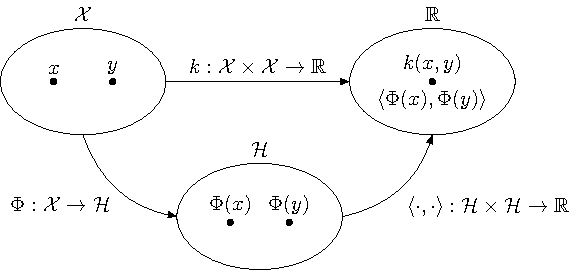
\includegraphics[]{figs/fig-kernel-map-diagram}
    \caption{Kernel map diagram.}
    \label{fig:kernel-map-diagram}
\end{figure}

\paragraph{Constructing a feature map.}
\def\Ho{H_0}
\def\iptHo#1{\ipt{#1}_{\Ho}}

Consider the map\footnote{
    Here, \(\Phi : \X \to (\X \to \RR)\) is just the \textit{curried} form of the binary function \(k : \X \times \X \to \RR\).
    For example, \(\{k(x, \cdot) \mid x \in \X\}\) describes a set of unary functions curried from the binary function \(k\).
} \(\Phi(x) = k(x, \cdot)\), for all \(x \in \X\).
Note that by the symmetry of \(k\), we can write \(\Phi(x) = k(x, \cdot) = k(\cdot, x)\).
Taking the linear span of \(\Phi(\X)\) gives us
\begin{equation}
    \Ho = \lspan \Phi(\X)
    = \left\{
        f = \sum_{i=1}^{n} \alpha_i k(x_i, \cdot)
        \;\middle|\;
        \begin{aligned}
            \forall n &\in \NN,\\
            x_1, x_2, \dots, x_n &\in \X,\\
            \alpha_1, \alpha_2, \dots, \alpha_n &\in \RR
        \end{aligned}
    \right\},
\end{equation}
which forms a subspace of \(\RR^{\X}\).
By \Cref{def:feature-map}, \(\Ho\) is a feature space.

\paragraph{Constructing an inner product.}

Let \(f,g \in \Ho\).
Then there exist \(n, m \in \NN\), \((\alpha_i)_{i=1}^n\), \((\beta_j)_{j=1}^m\), \((x_i)_{i=1}^n\), \((y_j)_{j=1}^m\) such that
\begin{equation}
    \label{eqn:function-linear-combo}
    f = \sum_{i=1}^{n} \alpha_i k(x_i, \cdot)
    \quad\text{and}\quad
    g = \sum_{j=1}^{m} \beta_j k(y_j, \cdot).
\end{equation}
Define \(\iptHo{\cdot, \cdot} : \Ho \times \Ho \to \RR\) as
\begin{equation}
    \label{eqn:pre-hilbert-inner-product}
    \iptHo{f, g} 
    = \sum_{i=1}^{n} \sum_{j=1}^{m} \alpha_i \beta_j k(x_i, y_j).
\end{equation}
Letting \(m=1\), \(\beta_1=1\), \(y_1 = y\) in \cref{eqn:function-linear-combo,eqn:pre-hilbert-inner-product}, then \(g = k(y,\cdot)\).
This shows that \(k\) has the \textit{reproducing property}
\begin{equation}
    \label{eqn:reproducing-property}
    \iptHo{f, k(y, \cdot)} = \sum_{i=1}^{n} \alpha_i k(x_i, y) = f(y),
\end{equation}
for all \(y \in \X\).
Similarly, letting \(n=1\), \(\alpha_1=1\), \(x_1=x\), we have
\begin{equation}
    \label{eqn:kernel-is-inner-product}
    k(x,y) = \iptHo{k(x,\cdot), k(y,\cdot)} = \iptHo{\Phi(x), \Phi(y)},
\end{equation}
for all \(x,y \in \X\).
Now we will show that \(\iptHo{\cdot, \cdot}\) is an inner product.
\begin{enumerate}
    \item Since \(k\) is symmetric, we have
    \begin{equation}
        \iptHo{f, g}
        = \sum_{i=1}^{n} \sum_{j=1}^{m} \alpha_i \beta_j k(x_i, y_j)
        = \sum_{j=1}^{m} \sum_{i=1}^{n} \beta_j \alpha_i k(y_j, x_i)
        = \iptHo{g, f}.
    \end{equation}
    \item By rearrangement, \cref{eqn:pre-hilbert-inner-product} becomes
    \begin{equation}
        \iptHo{f, g}
        % = \sum_{i=1}^{n} \sum_{j=1}^{m} \alpha_i \beta_j k(x_i, y_j)
        = \sum_{j=1}^{m} \beta_j \sum_{i=1}^{n} \alpha_i k(x_i, y_j)
        = \sum_{j=1}^{m} \beta_j f(y_j).
    \end{equation}
    Then for all \(f_1, f_2 \in \lspan \Phi(\X)\) and \(\alpha, \gamma \in \RR\),
    \begin{align}
            \iptHo{\alpha f_1 + \gamma f_2, g}
            &= \sum_{j=1}^{m} \beta_j (\alpha f_1 + \gamma f_2)(y_j) \\
            &= \alpha \sum_{j=1}^{m} \beta_j f_1(y_j) + \gamma \sum_{j=1}^{m} \beta_j f_2(y_j)
            \notag\\
            &= \alpha \iptHo{f_1, g} + \gamma \iptHo{f_2, g}.
            \notag
    \end{align}
    \item Since \(k\) is positive semidefinite, by \Cref{lem:properties-of-kernels} \cref{itm:properties-of-kernels-psd}
    \begin{equation}
        \iptHo{f,f}
        = \sum_{i=1}^{n} \sum_{j=1}^{n} \alpha_i \alpha_j k(x_i, x_j)
        % = a^\top K a
        \geq 0.
    \end{equation}
    Now let \(f_1, f_2, \dots, f_p\) be functions and \(\gamma_1, \gamma_2, \dots, \gamma_p \in \RR\).
    Then by bilinearity,
    \begin{equation}
        \sum_{i=1}^{p} \sum_{j=1}^{p} \gamma_i \gamma_j \iptHo{f_i, f_j}
        = \iptHo{\sum_{i=1}^{p} \gamma_i f_i, \sum_{j=1}^{p} \gamma_j f_j}
        \geq 0.
    \end{equation}
    Thus, \(\iptHo{\cdot, \cdot}\) is a kernel.
    Then by \cref{eqn:reproducing-property} and \Cref{lem:properties-of-kernels} \cref{itm:properties-of-kernels-csi},
    \begin{equation}
        f(x)^2 = \iptHo{f, k(x, \cdot)}^2 \leq \iptHo{f,f} \iptHo{k(x, \cdot), k(x, \cdot)},
    \end{equation}
    for all \(x \in \X\).
    If \(\iptHo{f,f} = 0\), then \(f(x)^2 = 0\) implies \(f = 0\).
\end{enumerate}

\paragraph{Constructing a Hilbert space.}
\def\iptH#1{\ipt{#1}_{\H}}
Now that we know \(\iptHo{\cdot, \cdot}\) is an inner product, \(\Ho\) is an inner product space.
By \cite{kreyszig1991introductory}, this can be completed with respect to the induced metric.
Then
\begin{equation}
    \label{eqn:complete-feature-space}
    \H
    % = \overline{\Ho}
    = \overline{\lspan \Phi(\X)}
    = \overline{\lspan\{k(x, \cdot) \mid x \in \X\}}
\end{equation}
is a Hilbert space with inner product \(\iptH{\cdot, \cdot} : \H \times \H \to \RR\).
Since \(\H\) contains all its limit points, functions in this space have the form
the sequences \((\alpha_i)_{i=1}^\infty\) and \((x_i)_{i=1}^\infty\) determine a function \(f \in \H\) such that
\begin{equation}
    f = \sum_{i=1}^{\infty} \alpha_i k(x_i, \cdot),
\end{equation}
provided the series converges.